\documentclass[12pt, a4paper, oneside, UTF8]{ctexart}
\usepackage{amsmath, amsthm, amssymb, bm, color, framed, graphicx, hyperref, mathrsfs}
\usepackage{geometry}
\geometry{left = 2.5 cm, right = 2.5 cm, top = 2.5 cm, bottom = 2.5 cm}

\title{\textbf{作业8}\\{\small (数值算法与案例分析)}}
\author{李维杰}
\date{\today}
\linespread{1.5}
\definecolor{shadecolor}{RGB}{241, 241, 255}
\newcounter{problemname}
\newenvironment{problem}{\begin{shaded}\stepcounter{problemname}\par\noindent\textbf{题目\arabic{problemname}. }}{\end{shaded}\par}
\newenvironment{solution}{\par\noindent\textbf{解答. }}{\par}
\newenvironment{note}{\par\noindent\textbf{注记. }}{\par}

\begin{document}

\maketitle

\begin{problem}
    设$A \in \mathbb{C}^{n \times n}, x \in \mathbb{C}^{n}$.假设$X = [x, Ax, ..., A^{n-1}x]$是非奇异的.\\
    证明: $X^{-1}AX$ 是一个上Hessenberg阵.
\end{problem}

\begin{solution}
    设$X^{-1}AX=H$,其中$H=(h_{i,j})$.则有$AX=XH$,即
    \begin{align*}
        \left[
            \begin{array}{cccc}
                Ax & A^{2}x  & ...  & A^{n}x
            \end{array}
        \right] = 
        \left[
            \begin{array}{cccc}
                x & Ax  & ...  & A^{n-1}x
            \end{array}
        \right]
        H .
    \end{align*}
    进一步展开,即得
    \begin{align*}
        A^{k}x=\sum\limits_{i=1}^{n}{h_{i,k}A^{i-1}x}.
    \end{align*}
    由于$X$是非奇异的,故$x,Ax,...,A^{n-1}x$线性无关.则由上式可以直接得出
    \begin{align*}
        \left\{
            \begin{array}{ll}
                h_{i,k}=1 , i = k+1 \\
                h_{i,k}=0 , i \neq k+1
            \end{array}
        \right. , k = 1,2,...,n-1.
    \end{align*}
    故
    \begin{align*}
        H = \left[
            \begin{array}{ccccc}
                0 & 0 & \cdots & 0 & h_{1,n} \\
                1 & 0 & \cdots & 0 & h_{2,n} \\
                0 & 1 & \cdots & 0 & h_{3,n} \\
                \vdots & \vdots & \ddots & \vdots & \vdots \\
                0 & 0 & \cdots & 1 & h_{n,n}
            \end{array}
        \right] ,
    \end{align*}
    这是一个上Hessenberg阵.
\end{solution}

\begin{problem}
    设$A \in \mathbb{C}^{n \times n}$是一个未缩减的上Hessenberg阵.其中未缩减的意思是对于$1 \leqslant i \leqslant n-1$,均有$A_{i+1,i} \neq 0$.假设$A$是奇异的.\\
    证明: $0$ 特征值将在一步$QR$迭代后出现在矩阵的右下角.\\
    另外考虑:保持$A$是一个奇异的上Hessenberg阵.当某些$A_{i+1,i}=0$时会出现什么状况?
\end{problem}

\begin{solution}
    由于$A$是奇异的,则对$A$做$QR$分解后,可得分块矩阵$Q= \left[ \begin{array}{cc} \tilde{Q} & 0 \end{array} \right]$和$R = \left[ \begin{array}{cc} \tilde{R} \\ 0 \end{array} \right]$.
    故一步迭代后,即得
    \begin{align*}
        A' = RQ = \left[ \begin{array}{cc} \tilde{Q}\tilde{R} & 0 \\ 0 & 0\end{array} \right] .
    \end{align*}
    也即$0$特征值将出现在一步迭代后矩阵的右下角.\\
    当存在某些$A_{i+1,i}=0$时,若采用Givens变换不断消去bulge的算法进行QR分解,则算法会在$G(i,i+1)$处中断导致迭代无法完成.
    故此时必须采用其它QR分解的算法(如MGS等)对A进行QR分解,同上述证明可得$0$特征值会出现在一步迭代后矩阵的右下角.
\end{solution}

\begin{problem}
    设
    \begin{align*}
        A = 
        \left[
            \begin{array}{ccccc}	
                0 &   &   &   & 1 \\
                1 & 0 &   &   &   \\
                  & \ddots & \ddots &   & \\
                  &   & 1 & 0 & \\
                  &   &   & 1 & 0 
            \end{array}
        \right] .
    \end{align*}
    试评价下面两种算法作用于该矩阵时的收敛性情况:\\
    (1) 朴素QR算法,\\
    (2) Francis' double-shift QR算法.
\end{problem}

\begin{solution}
    (1) 注意到$A$的一个QR分解就是$A = AI$,则一步迭代后变为$A^{(1)} = IA = A$, 故该矩阵在朴素QR算法下不会收敛.\\
    (2) 由于矩阵$A$上Hessenberg化后仍为矩阵$A$,其右下角$2 \times 2$子矩阵$\left[ \begin{array}{cc} 0 & 0 \\ 1 & 0 \end{array} \right]$的特征值为$0$,
    则对该矩阵使用Francis' double-shift QR算法的第一步迭代等价于朴素QR分解,由(1)知朴素QR迭代过程不会改变矩阵$A$,故在Francis' double-shift算法下该矩阵同样不会收敛.
\end{solution}
\newpage
\begin{problem}
    设
    \begin{align*}
        A = 
        \left[
            \begin{array}{cc}	
                a & c \\
                0 & b
            \end{array}
        \right] \in \mathbb{R}^{2 \times 2}.
    \end{align*}
    设计一个算法来生成一个正交矩阵$Q$,使得
    \begin{align*}
        Q^{T}AQ = 
        \left[
            \begin{array}{cc}	
                b & c \\
                0 & a
            \end{array}
        \right] .
    \end{align*}
\end{problem}

\begin{solution}
    设$Q=\left[ \begin{array}{cc} \cos{\theta} & -\sin{\theta} \\ \sin{\theta} & \cos{\theta} \end{array} \right]$,则
    \begin{align*}
        Q^{T}AQ = \left[ 
            \begin{array}{cc} 
                a\cos^2{\theta}+b\sin^2{\theta}+c\sin{\theta}\cos{\theta} & -a\sin{\theta}\cos{\theta}+b\sin{\theta}\cos{\theta}+c\cos^2{\theta} \\ 
                -a\sin{\theta}\cos{\theta}+b\sin{\theta}\cos{\theta}-c\sin^2{\theta} & a\sin^2{\theta}+b\cos^2{\theta}-c\sin{\theta}\cos{\theta}
            \end{array} 
        \right] .
    \end{align*}
    于是有方程组:
    \begin{align*}
        \left\{
            \begin{array}{llll}
                a\cos^2{\theta}+b\sin^2{\theta}+c\sin{\theta}\cos{\theta} = b \\
                -a\sin{\theta}\cos{\theta}+b\sin{\theta}\cos{\theta}+c\cos^2{\theta} = c \\
                -a\sin{\theta}\cos{\theta}+b\sin{\theta}\cos{\theta}-c\sin^2{\theta} = 0 \\
                a\sin^2{\theta}+b\cos^2{\theta}-c\sin{\theta}\cos{\theta} = a
            \end{array}
        \right. ,
    \end{align*}
    解此方程组,得$\tan{\theta} = \frac{b-a}{c}$,也即
    \begin{align*}
        \left\{
            \begin{array}{ll}
                \sin{\theta} = \frac{b-a}{\sqrt{(b-a)^2+c^2}} \\
                \cos{\theta} = \frac{c}{\sqrt{(b-a)^2+c^2}}
            \end{array}
        \right. .
    \end{align*}
    由此即可生成符合题意的$Q$.随机生成$10$个矩阵$A$,并设$\tilde{A} = \left[ \begin{array}{cc} b & c \\ 0 & a \end{array} \right]$,由上述算法确定$Q$,计算相应的${\left\lVert{Q^{T}AQ-\tilde{A}}\right\rVert}_{\mathsf{F}}$如下图
    (代码见Problem4.m)
    \begin{figure}[htbp] % 创建一个图形环境
        \centering % 图片居中
        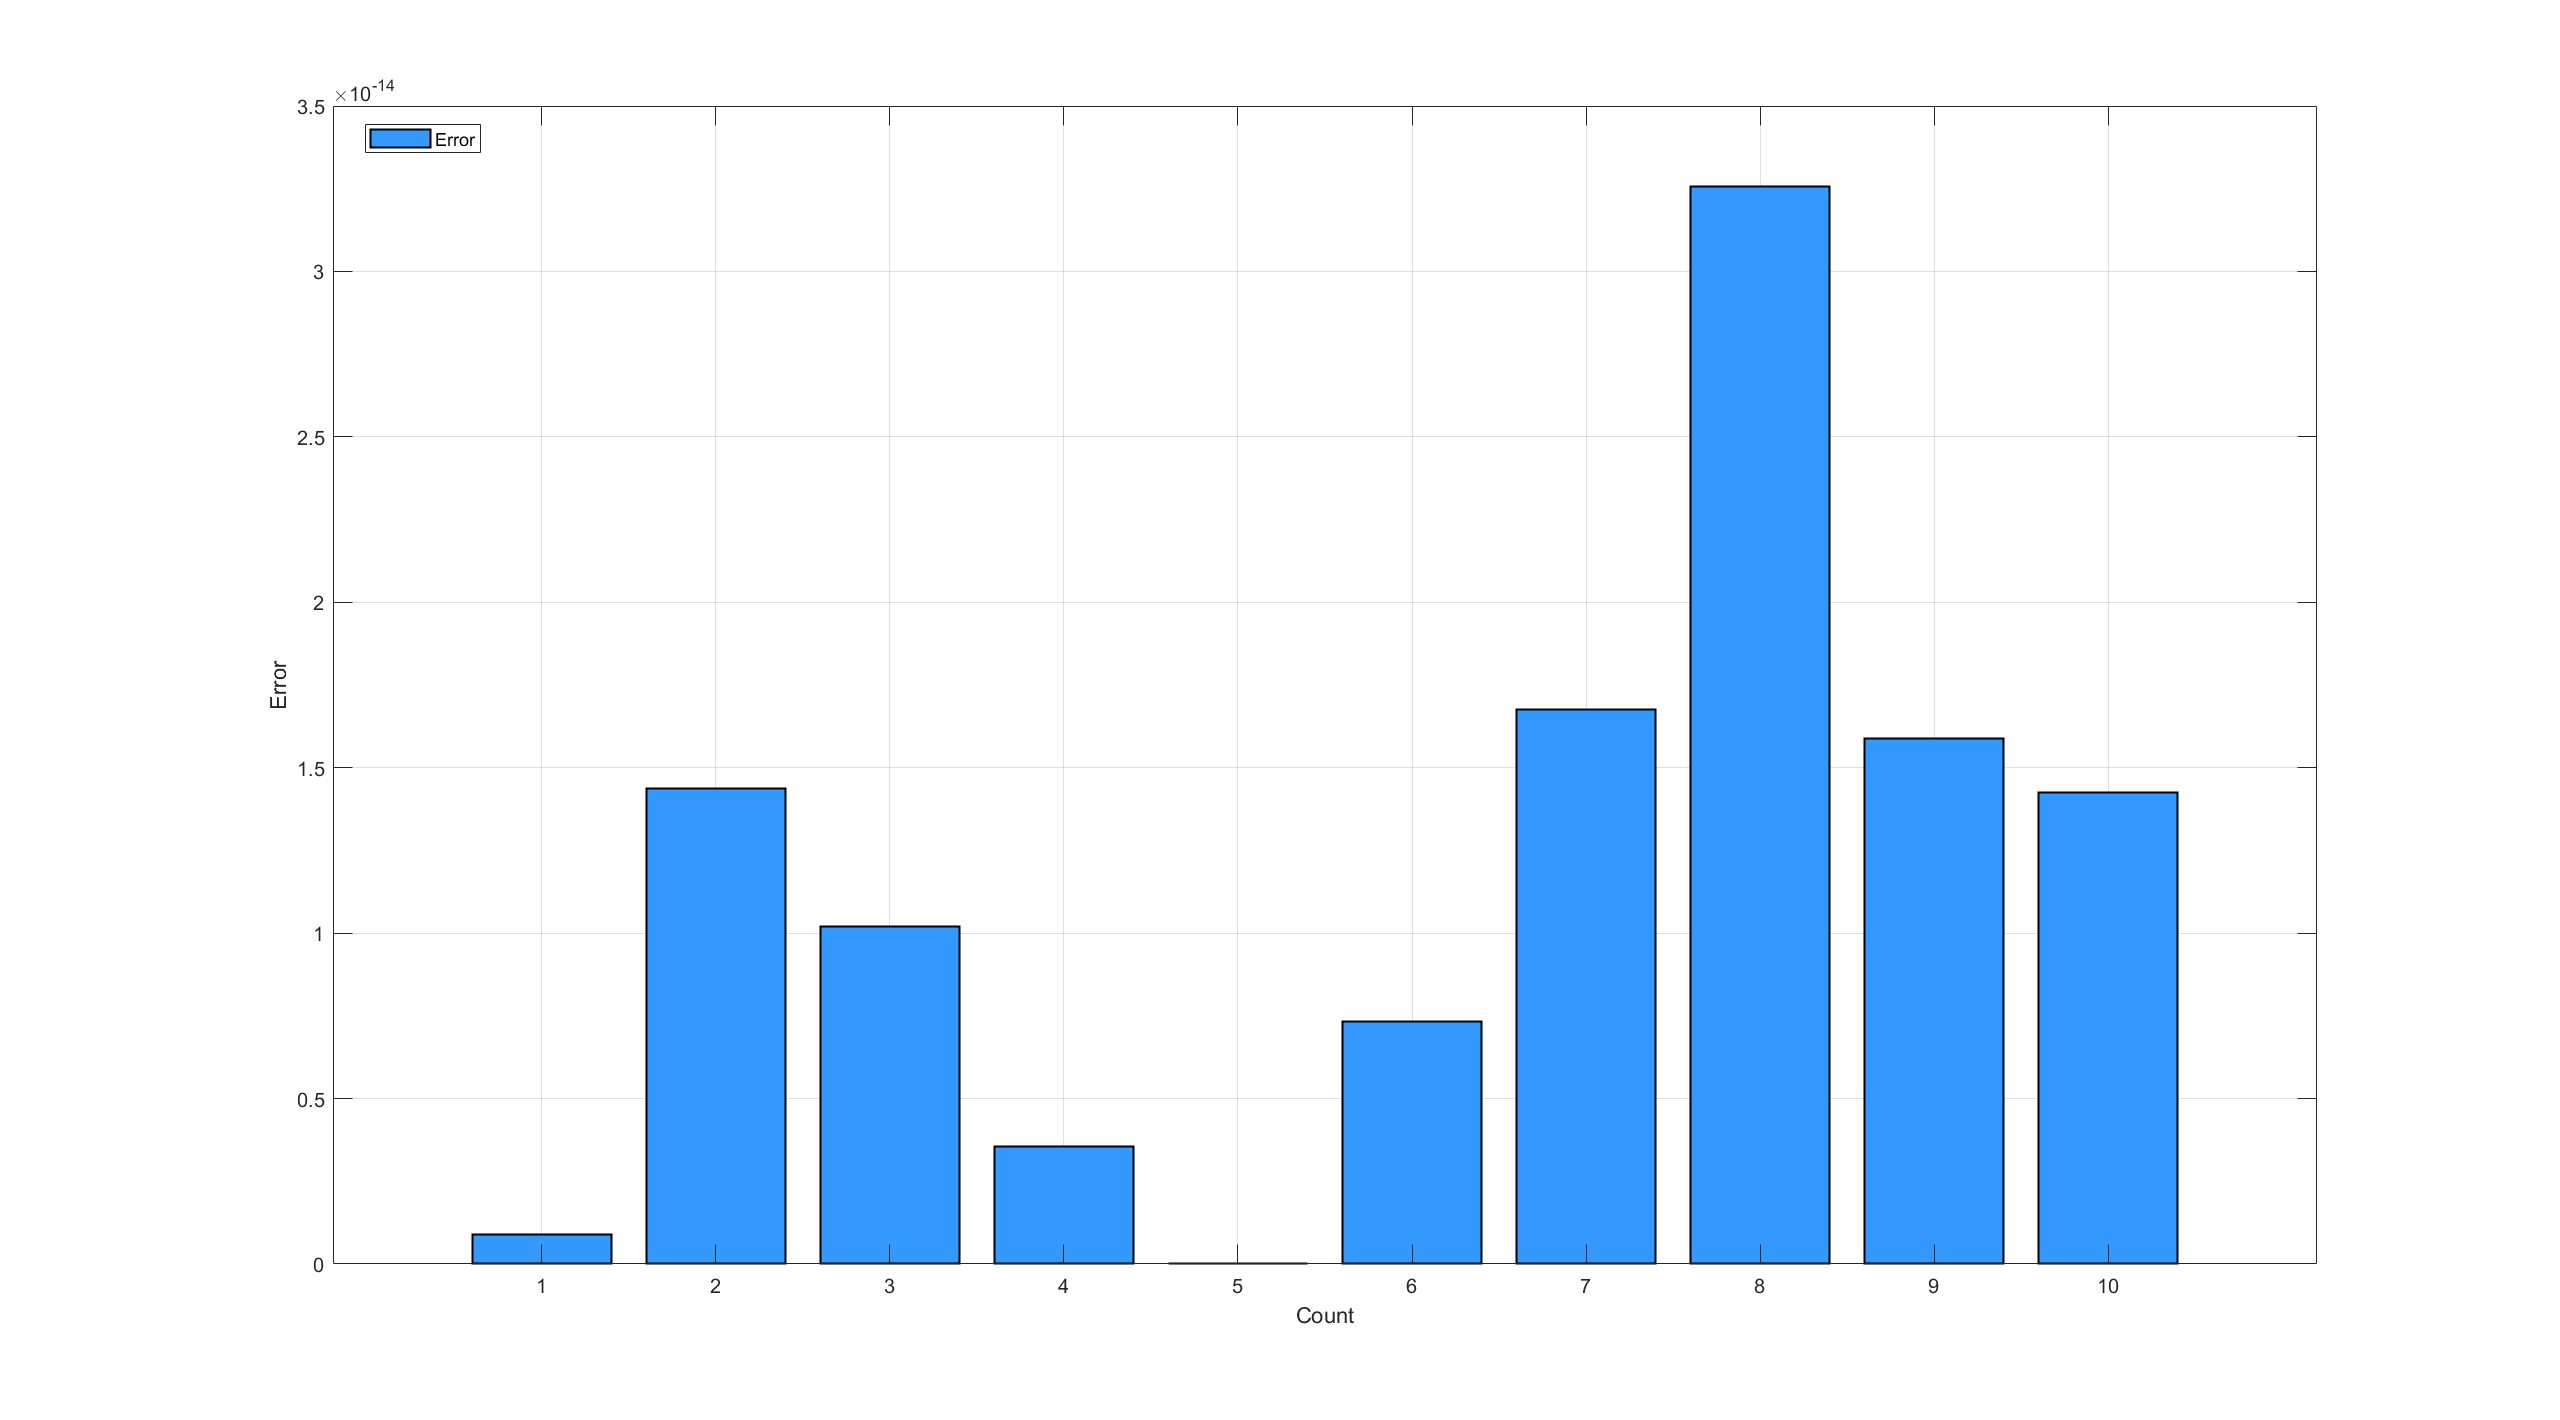
\includegraphics[scale=0.14]{Problem4.jpg} % 插入图片,设置宽度为页面宽度的70%
        \caption{对$A$进行正交相似变换后与目标矩阵$\tilde{A}$之间的误差} % 图片的说明文字
    \end{figure}
\end{solution}
\newpage
\begin{problem}
    执行下列用于矩阵上Hessenberg化的算法:\\
    (a) 使用Householder reflections;\\
    (b) 使用基于MGS正交化的Arnoldi变换.\\
    随机生成一些矩阵并计算相应的Hessenberg分解 $A=QHQ^{*}$.通过计算${\left\lVert{Q^{*}AQ-H}\right\rVert}_{\mathsf{F}}$ 和 ${\left\lVert{Q^{*}Q-I}\right\rVert}_{\mathsf{F}}$来检查程序的准确性.并说明有什么发现.
\end{problem}

\begin{solution}
    (代码见Problem5.m)
    \begin{figure}[htbp] % 创建一个图形环境
        \centering % 图片居中
        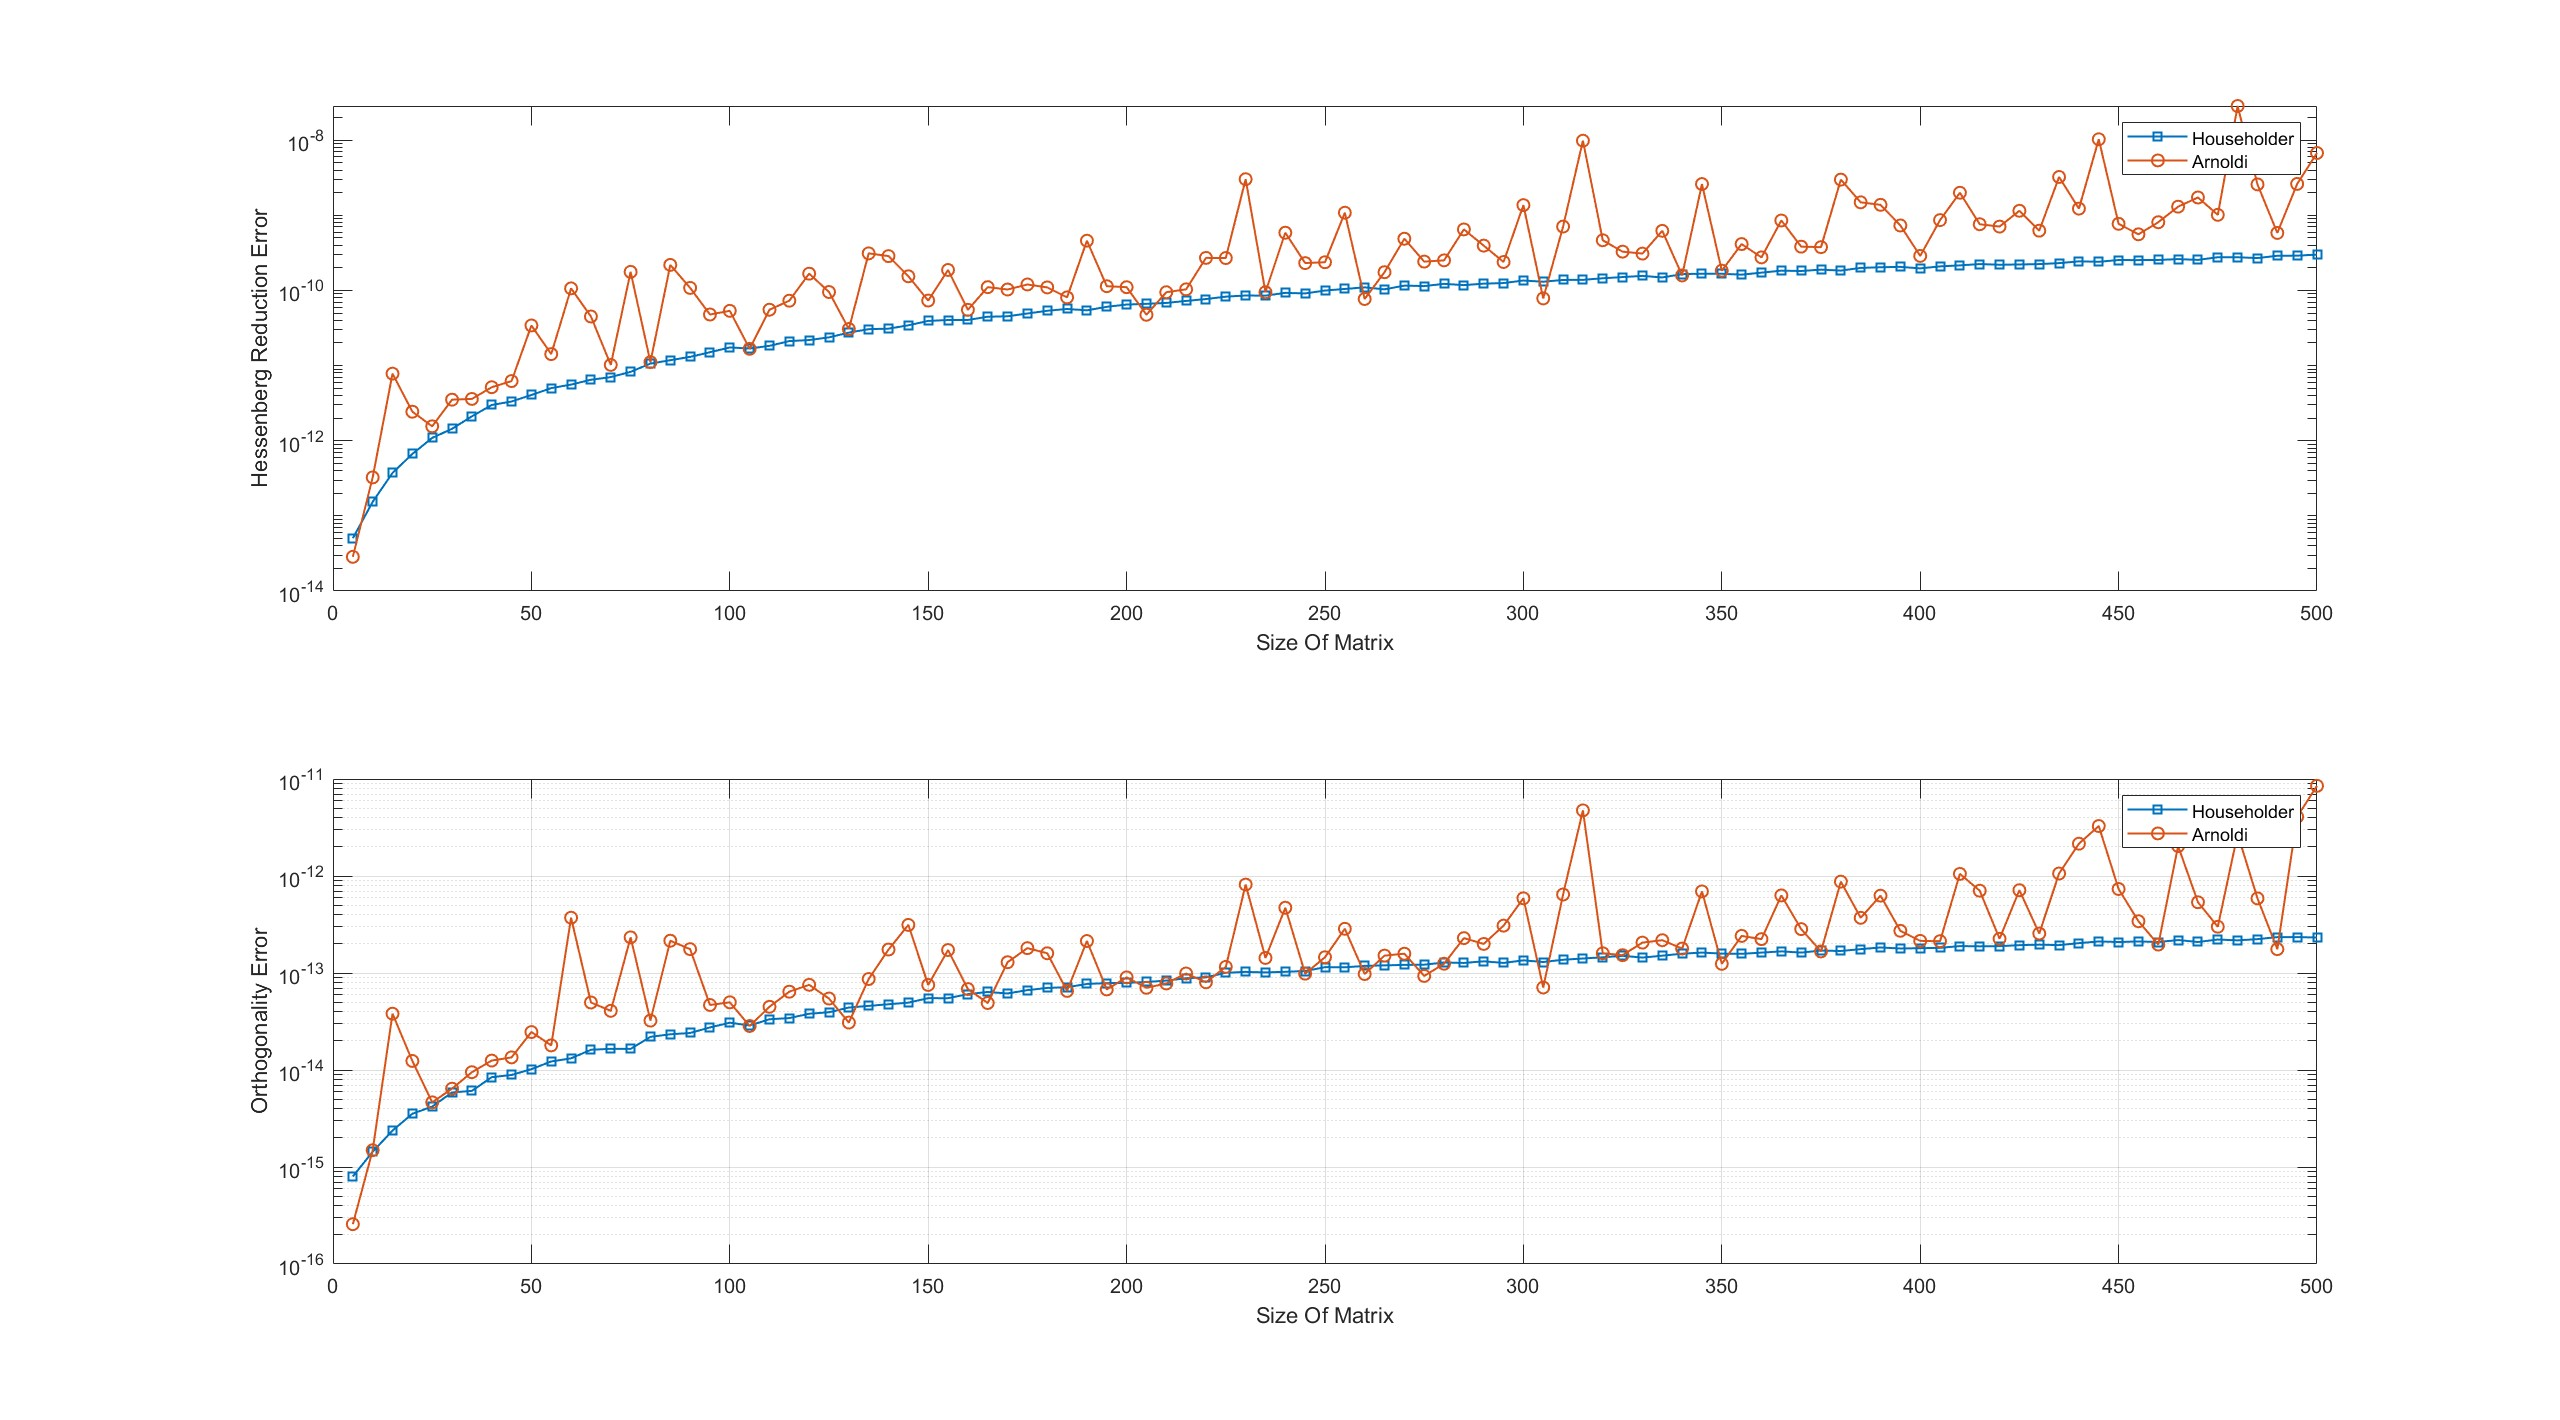
\includegraphics[scale=0.14]{Problem5.jpg} % 插入图片,设置宽度为页面宽度的70%
        \caption{两种算法的误差表现} % 图片的说明文字
    \end{figure}\par
    由图知基于Householder变换的矩阵上Hessenberg化算法具有更小的误差和更优越的稳定性.
\end{solution}

\end{document}